% Figure 3 of docs/exposition.md: the two reflections of amplitude
% amplification in the plane of the acceptance direction g and the rejection
% direction b, drawn for theta = 20 degrees. Uses the palette of style.tex.
% Build with tools/render_papers.py.
\documentclass[tikz,border=4pt]{standalone}
% Shared TikZ style for the figures of docs/exposition.md.
% Palette and bit cells follow docs/figures/expert_column.tex.
\usepackage{amsmath,amssymb}
\usetikzlibrary{arrows.meta,positioning,calc,decorations.pathreplacing}
\definecolor{one}{RGB}{226,232,240}
\definecolor{zero}{RGB}{40,40,40}
\definecolor{win}{RGB}{176,58,46}
\definecolor{addr}{RGB}{40,90,150}
\definecolor{lose}{RGB}{110,110,110}
\tikzset{
  bit/.style={draw=black!60, minimum width=4.4mm, minimum height=4.4mm,
              inner sep=0pt, font=\scriptsize},
  onebit/.style={bit, fill=one},
  zerobit/.style={bit, fill=zero, text=white},
  cell/.style={draw=black!50, fill=white, minimum width=10mm,
               minimum height=4.2mm, inner sep=0pt, font=\scriptsize},
  >={Stealth[length=2.2mm]}}

% \boardcolumn{name}{x}{b1}{b2}{b3}{b4}{address text}
% Draws X_name as four bits at height 0 starting at x, the address inputs
% below, and the four cells 00,01,10,11 named <name>c00 ... <name>c11.
\newcommand{\boardcolumn}[7]{%
  \node[anchor=east, font=\small] at (#2-0.05,0) {$X_{#1}$};
  \foreach \c/\b in {1/#3,2/#4,3/#5,4/#6} {
    \ifnum\b=0
      \node[zerobit] (x#1-\c) at (#2+0.46*\c-0.23,0) {0};
    \else
      \node[onebit] (x#1-\c) at (#2+0.46*\c-0.23,0) {1};
    \fi}
  \node[font=\small, align=center, addr, anchor=north] (adr#1)
    at (#2+0.92,-0.38) {#7};
  \foreach \s/\k in {00/0,01/1,10/2,11/3} {
    \node[cell] (#1c\s) at (#2+0.92,-1.62-0.5*\k) {$B_{#1,\s}$};}
}

\begin{document}
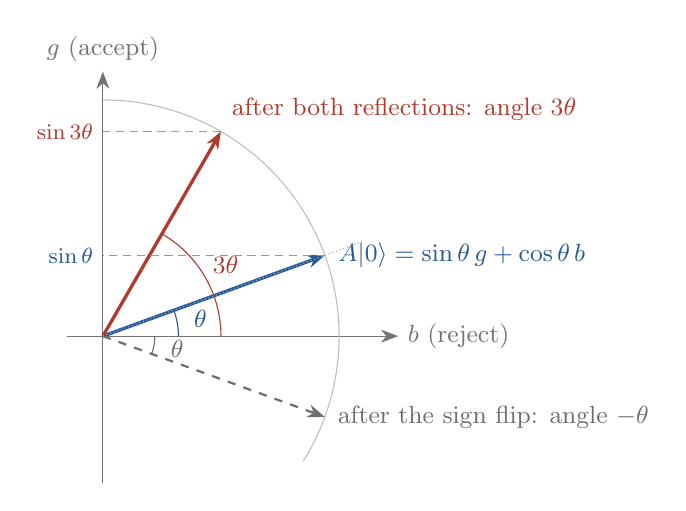
\begin{tikzpicture}[scale=3.0, font=\small]
\def\th{20}
% axes and unit arc
\draw[->, black!55] (-0.15,0) -- (1.25,0) node[right] {$b$ (reject)};
\draw[->, black!55] (0,-0.62) -- (0,1.12) node[above] {$g$ (accept)};
\draw[black!25] (1,0) arc[start angle=0, end angle=90, radius=1];
\draw[black!25] (1,0) arc[start angle=0, end angle=-32, radius=1];
% prepared state at angle theta
\draw[->, very thick, addr] (0,0) -- (\th:1) node[right=1pt] {$A|0\rangle=\sin\theta\,g+\cos\theta\,b$};
% after the sign flip: angle -theta
\draw[->, thick, lose, dashed] (0,0) -- (-\th:1) node[right=1pt] {after the sign flip: angle $-\theta$};
% after reflecting about the prepared state: angle 3 theta
\draw[->, very thick, win] (0,0) -- (3*\th:1) node[above right=0pt] {after both reflections: angle $3\theta$};
% the mirror line through the prepared state
\draw[addr!50, densely dotted] (0,0) -- (\th:1.18);
% angle marks
\draw[addr] (0.32,0) arc[start angle=0, end angle=\th, radius=0.32];
\node[addr] at (\th/2:0.42) {$\theta$};
\draw[lose] (0.22,0) arc[start angle=0, end angle=-\th, radius=0.22];
\node[lose] at (-\th/2:0.32) {$\theta$};
\draw[win] (0.5,0) arc[start angle=0, end angle=3*\th, radius=0.5];
\node[win] at (1.5*\th:0.6) {$3\theta$};
% projection onto g: the acceptance amplitude
\draw[win!60, densely dashed] (3*\th:1) -- (0,{sin(3*\th)});
\node[win, anchor=east, font=\footnotesize] at (0,{sin(3*\th)}) {$\sin3\theta$};
\draw[addr!60, densely dashed] (\th:1) -- (0,{sin(\th)});
\node[addr, anchor=east, font=\footnotesize] at (0,{sin(\th)}) {$\sin\theta$};
\end{tikzpicture}
\end{document}
